\subsection{[Matti] SVM}

\subsubsection{General notes}
\begin{itemize}
\item Number of bins for the ROC curve is 100, and specified in
  \texttt{src/Config.cxx} under the TMVA source tree.
  \begin{itemize}
  \item This can be changed by \texttt{TMVA::gConfig().GetVariablePlotting().fNbinsXOfROCCurve = 1000;}
  \item It looks like when the ROC curve is constructed (in
    \texttt{src/MethodBase.cxx}; except for Cuts), the background
    efficiency is interpolated with splines from a histogram with
    $10^4$ bins. The histogram in question is the bacgkround
    efficiency as a function of discriminator value
  \item It could be possible to recompute the ROC curve in a plotting
    script (except for Cuts)
  \item The whole thing is probably not a problem, since the
    background efficiency is floating point number
  \end{itemize}
%\item All variables (branches) in the tree are float, right? \textbf{Yes}
\item Signal and background event weights are now both 1. This should
  probably be fixed; is hardcoding to \texttt{code/chep09tmva} ok or
  do we want it to be a configuration parameter?
\item The normalization mode should be checked(NormMode parameter for
  the trainer, currently it has the value NumEvents), also the
  SplitMode (now Random) might not be good
%\item In the case that the big data is in madhatter, we should use
%  ametisti (or sepeli). I think we should at least discuss about the
%  possibility of having the data in ametisti instead of madhatter.
\item The \texttt{TestTree} tree in output \texttt{TMVA.root} can be
  used to see the output distributions of the variables after placing
  a cut on the classifier discriminator
  \begin{itemize}
  \item The branch \texttt{type} seems to be 0 for background and 1 for signal
  \end{itemize}
\item What number(s) should we look when optimizing the classifier?
  \begin{itemize}
  \item Signal efficiency at $10^5$ background rejection?
  \end{itemize}
\item What to do with the random number seed problem we had last time?
  \begin{itemize}
  \item The training of some classifiers depends highly on the random
    number generator(s). There is really no global random number seed,
    so the training might be in general indeterministic with respect
    to the parameters of the classifier.
  \item Few options comes to my mind:
    \begin{itemize}
    \item[a)] Try to look the average training behaviour by training
      several classifiers with same parameters by (somehow) varying
      the random number seed.
    \item[b)] Choose the parameters with which the classifier
      performance is best
    \end{itemize}
  \end{itemize}
\item It seems that the Cuts classifier evaluation time scales
  quadratically w.r.t the size of the test tree. (Our event evalution
  with \texttt{MyEvaluate} has linear scaling.)% This behaviour is
  %demonstrated in table~\ref{table:mkCutsScaling} and in
  %figure~\ref{fig:mkCutsScaling}.
  Other classifiers might not be incluenced by this, as is
  demonstrated in the table with SVM.

  \textbf{Update 2009-02-05:} This seems to be affected also by the
  (background) data. When the jets with $\texttt{jeteta}=0$ are
  removed, Cuts classifier gets evaluated also in reasonable time
  (faster than in \texttt{MyEvaluate}).
\end{itemize}

% \begin{table}
%   \caption{Comparison of TMVA evaluation to our event
%     testing+evaluation with Cuts and SVM classifiers. The numbers are
%     real time in seconds, and they are \textbf{suggestive only}.}
%   \label{table:mkCutsScaling}
%   \begin{center}
%     \begin{tabular}{c|cc|cc}
%       Training & \multicolumn{2}{|c|}{Cuts} & \multicolumn{2}{|c}{SVM} \\
%       jets     & TMVA test+eval. & Event eval.   & TMVA test+eval. & Event eval. \\
%       \hline
%       10000    & 0.43            & 1.13          & 0.67            & 0.73 \\
%       20000    & 1.53            & 1.75          & 1.21            & 1.53 \\
%       50000    & 12.1            & 4.04          & 2.15            & 2.03 \\
%       80000    & 32.6            & 6.19          & 2.70            & 2.81 \\
%       100000   & 51.1            & 7.55          & 3.84            & 3.26 \\
%       150000   & 114             & 11.3          & 5.70            & 6.36 \\
%       200000   & 202             & 15.4          & 7.42            & 6.00 \\
%       250000   & 315             & 18.6          & 7.99            & 8.36 \\
%       300000   & 440             & 22.4          & 11.1            & 10.2 \\
%       400000   & 893             & 29.9          & 12.4            & 11.5 \\
%       500000   & 1560            & 38.8          & 18.3            & 16.2
%     \end{tabular}
%   \end{center}
% \end{table}

% \begin{figure}
%   \begin{center}
%     \begin{minipage}{.35\textwidth}
%       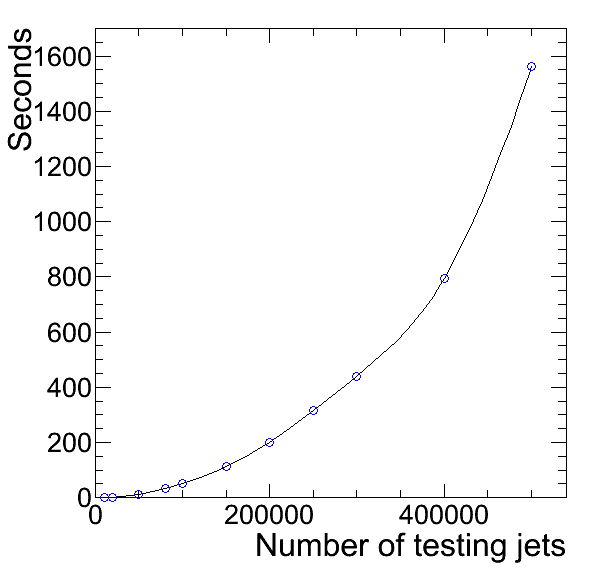
\includegraphics[width=\textwidth]{images/mkTmvaEval}
%     \end{minipage}
%     \hspace{.1\textwidth}
%     \begin{minipage}{.35\textwidth}
%       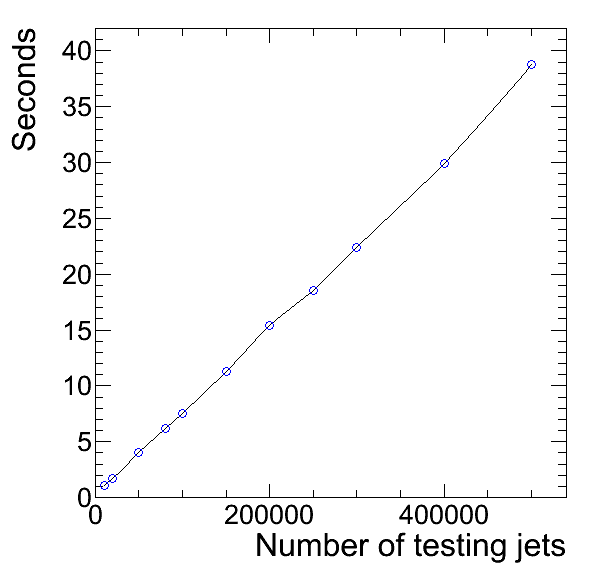
\includegraphics[width=\textwidth]{images/mkEventEval}
%     \end{minipage}
%   \end{center}
%   \caption{Real time spent in TMVA testing and evaluation together
%     (left) and in our event evaluation (right) as a function of
%     testing jets in input for Cuts classifier. The plots are
%     \textbf{suggestive only}, because they were produced from a single
%     run per data point and the reported time is real time.}
%   \label{fig:mkCutsScaling}
% \end{figure}


\subsubsection{Jet vs. event efficiencies}

\begin{itemize}
\item The input \texttt{TTree} for TMVA has jets as entries (i.e. TMVA
  ``event'' corresponds to a jet in the event generated in Pythia), so
  the efficiencies (and other quantities) reported by TMVA are for
  jets. The tree has branches for event and run numbers, so it is
  possible to separate the jets belonging to different events.
\item In the end, in order to have a physically reasonable result and
  to compare with other results, we would like to have the
  signal/background efficiencies of events, not jets (e.g. event is
  passed if there is at least one jet passing the classifier,
  otherwise the event is rejected)
\item In order to ``convert'' the jet efficiencies to event
  efficiencies, some kind of counting must be done
  \begin{enumerate}
  \item[a)] Optimisation is done only with jets, and for the final
    results the classifiers are used in event basis. Our abstract
    doesn't clearly specify, what we mean by $10^5$ background
    rejection (event vs. jet rejection).

  \item[b)] Use TMVA training tree for re-counting. However, the
    training tree contains only the variables used for training, and
    classifier outputs for the corresponding jets. In the current TMVA
    (v3.9.x) it seems to be impossible to add variables, which are not
    used for training/testing, to the training tree.

    It is of course possible to take the standalone TMVA as a part of
    our package and include this functionality. Actually, this has
    been requested in the TMVA users mailing list in 2007
    (\url{http://sourceforge.net/mailarchive/forum.php?thread_name=471C8D74.6040209\%40mpi-hd.mpg.de\&forum_name=tmva-users}),
    and it is in the TODO list
    (\url{http://tmva.cvs.sourceforge.net/tmva/TMVA/development/todo.txt?view=markup})
    with \emph{high priority}. Thus, my motivation of implementing
    this feature is not so high.

  \item[c)] Use the TMVA input tree for performing our own event-based
    counting. The TMVA preselection cuts and variable transformations
    will cause some headache, but it could be manageable. It might be
    easiest to take relevant pieces of code from TMVA and add glue,
    tape and gum to make it work. In order to not to use training data
    for testing, the training and testing trees should be in different
    files.
  \end{enumerate}
\item Currently (after commit
  82e7bc3d9575e853df7b65ebbbcdf5d91232802d) the event efficiencies are
  evaluated with the approach c). There are few things which should be
  noted in the current implementation
  \begin{description}
  \item[Training/test tree] The information about which jets are used
    for training by TMVA is not available (at least easily). Therefore
    the whole input tree is processed. This means, that if the one
    tree (or chain) is used for both training and testing in TMVA, the
    results produced by our evaluation code are biased. Fortunately, I
    think Lauri agreed about having the training and testing data in
    separate files (i.e. chains).

    The current code already supports separate chains for training and
    testing. If only training chain is defined (i.e. testing chain is
    empty), the training chain is used for both training and testing,
    as the situation was before.

  \item[Cuts vs. others] The signal/background efficiencies for other
    classifiers than cuts are produced with a code similar to the
    related code in TMVA, with the exception that only one jet per
    event is counted. However, Cuts classifier is a different story.

    The Cuts classifier is trained such that for each signal
    efficiency bin of ROC curve, TMVA maximizes the the background
    rejection. As some of the optimization algorithms have stochastic
    nature, the resulting ROC curve can have peaks. This means that
    for a given background efficiency level there might be multiple
    signal efficiencies (with different set of cuts, of course). TMVA
    chooses the smallest signal efficiency for their output, I've
    chosen the greatest (this also applies to other classifiers than
    Cuts, but for them I'd expect that ROC is smooth).

    Another difference comes from the fact that when other classifiers
    return a number which correlates with the probabability of the jet
    being $\tau$ jet, Cuts classifier returns boolean true/false
    (corresponding to a given signal efficiency). In order to test all
    trained cuts, all training signal efficiencies are looped over,
    and the TMVA reader is asked if the jet in question passes the
    cut. The number of passed events for each training signal
    efficiency is recorded, and with these \emph{true} signal and
    background efficiencies the ROC curve is constructed. The points
    with zero signal efficiency are not used, as they're probably just
    cases where the training has failed.

  \item[Reporting in output] The output of \texttt{chep09tmva} program
    became large, and it was also requested that it would be possible
    to switch \texttt{MyEvaluate} off. I added
    \texttt{AdditionalReports} section to the configuration file,
    where the possible reports can be switched on/off by
    (un)commenting the corresponding line. In the default
    configuration of \texttt{tmva-common.conf} and
    \texttt{tmva-example.conf} all reports are enabled.

  \item[Integration with TMVAGui.C?] Signal/background event
    efficiency histograms as well as the resulting ROC curves are
    stored to the output ROOT file. This enables the possibility to
    add these plots to the \texttt{TMVAGui.C} script.

    It should be noted that all other plots are histograms
    (\texttt{TH1}) except the ROC for Cuts, which is \texttt{TGraph}.

  \item[Maximum number of testing entries] \texttt{MyEvaluate} uses
    the same configuration as TMVA Factory (i.e. \texttt{NSigTest} and
    \texttt{NBkgTest} under \texttt{Trainer}) for specifying the
    maximum number of entries used for testing. If these are zero, all
    entries are used. It should be noted that unless both TMVA and
    \texttt{MyEvaluate} process the test trees entirely, they might
    process different entries.

  \item[Error estimation] Currently the reported errors come from the
    formula $\sigma=\sqrt{\varepsilon(1-\varepsilon)/N}$ as in TMVA.
    Should we also try to take the effect of binning into account?

  \end{description}
\end{itemize}

\subsubsection{SVM Notes}
%% \begin{itemize}
%% \item Training time scales as $O(n^2)$ where $n$ is the size of the
%%   input data (i.e. number of events)
%%   \begin{itemize}
%%   \item 100 signal and 200 background events took 0.125 seconds
%%   \item 200 signal and 400 background events took 0.542 seconds
%%   \item 500 signal and 1000 background events took 3.41 seconds
%%   \item 800 signal and 1600 background events took 10 seconds
%%   \item 1000 signal and 2000 background events took 13.8 seconds
%%   \item If the scaling law is correct, $10^4$ events would take about 2
%%     minutes, $5\times 10^4$ events would take almost an hour and $10^5$
%%     events would take more than 3,5 hours.
%%   \end{itemize}
%% \end{itemize}

\begin{itemize}
\item So far the best achieved signal event efficiency is $5.2\;\%$
  with parameters $\textrm{sigma}=4, \textrm{C}=7$.
\item The parameters for the best signal jet efficiency are
  $\textrm{sigma}=3,\textrm{C}=9$, which gives for event efficiency
  $4.6\;\%$. This shows that there is a difference between
  optimisation of jet and event efficiencies.
\end{itemize}

\subsubsection{TMVA Comments}
\begin{itemize}
\item The ROC curve for Cuts classifier is probably wrong. I guess
  that the signal efficiency comes from \textbf{training} and not from
  testing. For other classifiers the signal efficiency comes from
  testing.

  In the case of Cuts, also the background rejection could be wrong.
  E.g. it might happen that the cuts optimisation fails for some
  (training) signal efficiency or otherwise the cut values are
  non-valid. If this kind of cut is then applied to both signal and
  background data, nothing would be accepted, but in the ROC curve
  there is a rejection of 1 in the corresponding (training) signal
  efficiency bin.

\item There are a few special cases where the \emph{signal efficiency
    at bkg eff} numbers in the stdout could be wrong
  \begin{itemize}
  \item The achieved bacgkround efficiency is greater/smaller
    \emph{for all} signal efficiencies than the requested bkg eff
  \end{itemize}
\end{itemize}
